\documentclass[a4paper]{article}

\usepackage{siunitx}
\usepackage{graphicx}
\usepackage{hyperref}

\begin{document}
\title{Osborne 1 floppy drive emulator}
\date{July 2024}
\author{Archie Halliwell, Lennart Leufgens, Jun Muta}
\maketitle

\section{Introduction}

The Osborne 1 is a suitcase-sized portable computer released in 1981
is an important part in commputing history, being one of the first
widely available home computers. This project aims to allow the
sharing of programs for it over the internet. It replaces the floppy
disc module within the osborne with a small device that interfaces
with the motherboard and allows imagedisk files (.imd) to be
loaded. This replaces hard to find and costly 5.25'' floppy disks,
which need to be copied using legacy hardware, with usb drives, able
to be loaded with readily available files from the internet. The
entire project's source and documentation has been made readily
available on github
(\url{https://github.com/archiecarrot123/osborne-floppy-emulator}) for
anyone who desires to recreate this project.

\section{Repair}

A few weeks after we found the Osborne 1 in a cupboard, we decided to
plug it in and try to boot a floppy disk that said ``blank'' on
it. Around 30 seconds after we turned it on and tried to boot it, it
made a noise and we turned it off, after which it began emitting smoke
and we got Dr. Albrecht to take it away. After school, I took it home
to fix it. It turned out that this was a common issue caused by a
metallized paper capacitor absorbing so much moisture over the years
of being offline that it exploded. The replacement part was a
\qty{0.1}{\uF} X2 (line-to-line rated) capacitor from Jaycar, made of
metallised polypropylene. After replacing this capacitor I tried to
boot the Osborne again, and it started beeping loudly after trying to
load data off of the ``blank'' disk - later when probing the read data
line the signal from it seemed random, so it had probably either never
been written to or had an encounter with a magnet.

Much later, when checking the rotation rate of the floppy drives (I
had misunderstood the formatting and assumed that they must have a
rotation time of \qty{400}{\ms} instead of \qty{200}{\ms} to fit all
of the data), I discovered that the index pulse in drive 1 was not
working. After taking it apart, I found that the index pulse sensor
had broken off of the drive's chassis, but I glued it back together
and put it back and
then it worked.

\section{Hardware}

\subsection{SEPIC}

The first part of the floppy drive emulator that I designed was the
power supply, which was a single-ended primary inductor converter. The
reason why I chose to use a switchmode power supply was because I had
forgotten that the Osborne 1 supplies the disks with +5~V and I didn't
want to use a linear regulator to drop +12~V to +3.3~V as it would be
less than 30\% efficient. During my research into SMPSs I found that
the regular buck converter required either a P-channel MOSFET or a
N-channel MOSFET and a gate voltage above the input voltage, and the
other kinds of converters, such as the \v{C}uk converter that could
convert to a lower voltage using an N-channel MOSFET with a lower gate
voltage would produce a negative voltage. The SEPIC was the only
converter I saw that only used one diode and used a low-side N-channel
MOSFET.

I chose the value of the inductors using a formula I found in a book,
assuming a ripple current ratio of 0.4, \(V_{in}\) of \qty{12}{\V},
\(V_{out}\) of \qty{3.3}{\V}, and other parameters (frequency and
current) which I can't remember. I then created a schematic for the
converter using KiCad, and simulated it with Ngspice to fine tune
values.

I used a TL494 PWM control IC because it was available from Jaycar,
although it complicated the design as it was a TTL chip with two BJTs
as outputs, rather than a push-pull output which is suited to driving
the MOSFET. Because of this, I had to create my own MOSFET driver, but
because the IC had two outputs I could construct a simple push-pull
driver from one NPN and one PNP tranistor, as well as some resistors.

The SEPIC works by using the MOSFET (or other switching element) to
cause current to flow from the input through the input inductor, and
from the input side of the coupling capacitor, to ground. The current
flowing from the input side of the coupling capacitor also causes
current to flow from ground through the output inductor and into the
output side of the coupling capacitor. Then, when the MOSFET turns off
the current through the input inductor continues to flow, but now into
the input side of the coupling capacitor, causing current to flow out
of the output side and through the diode to the output; at the same
time current continues flowing from ground through the output
inductor, but now to the output through the diode. Because the current
waveforms through the inductors are the same, they can be wound on the
same core, which supposedly increases efficiency, and also reduces the
weight, though that isn't important here.

Because I was initially trying to do the project without buying many
components, I hand-wound two coupled inductors on the same core. Now
that I think of it, I could have wound them both at the same time but
for whatever reason I didn't think of that at the time. Once I figured
out that I would be best off buying components, I chose a \qty{1}{\uH}
SMD common-mode choke which, when flipped on its back, turned out to
contain a comically small toroid held in clear resin.

\begin{figure}
  \centering
  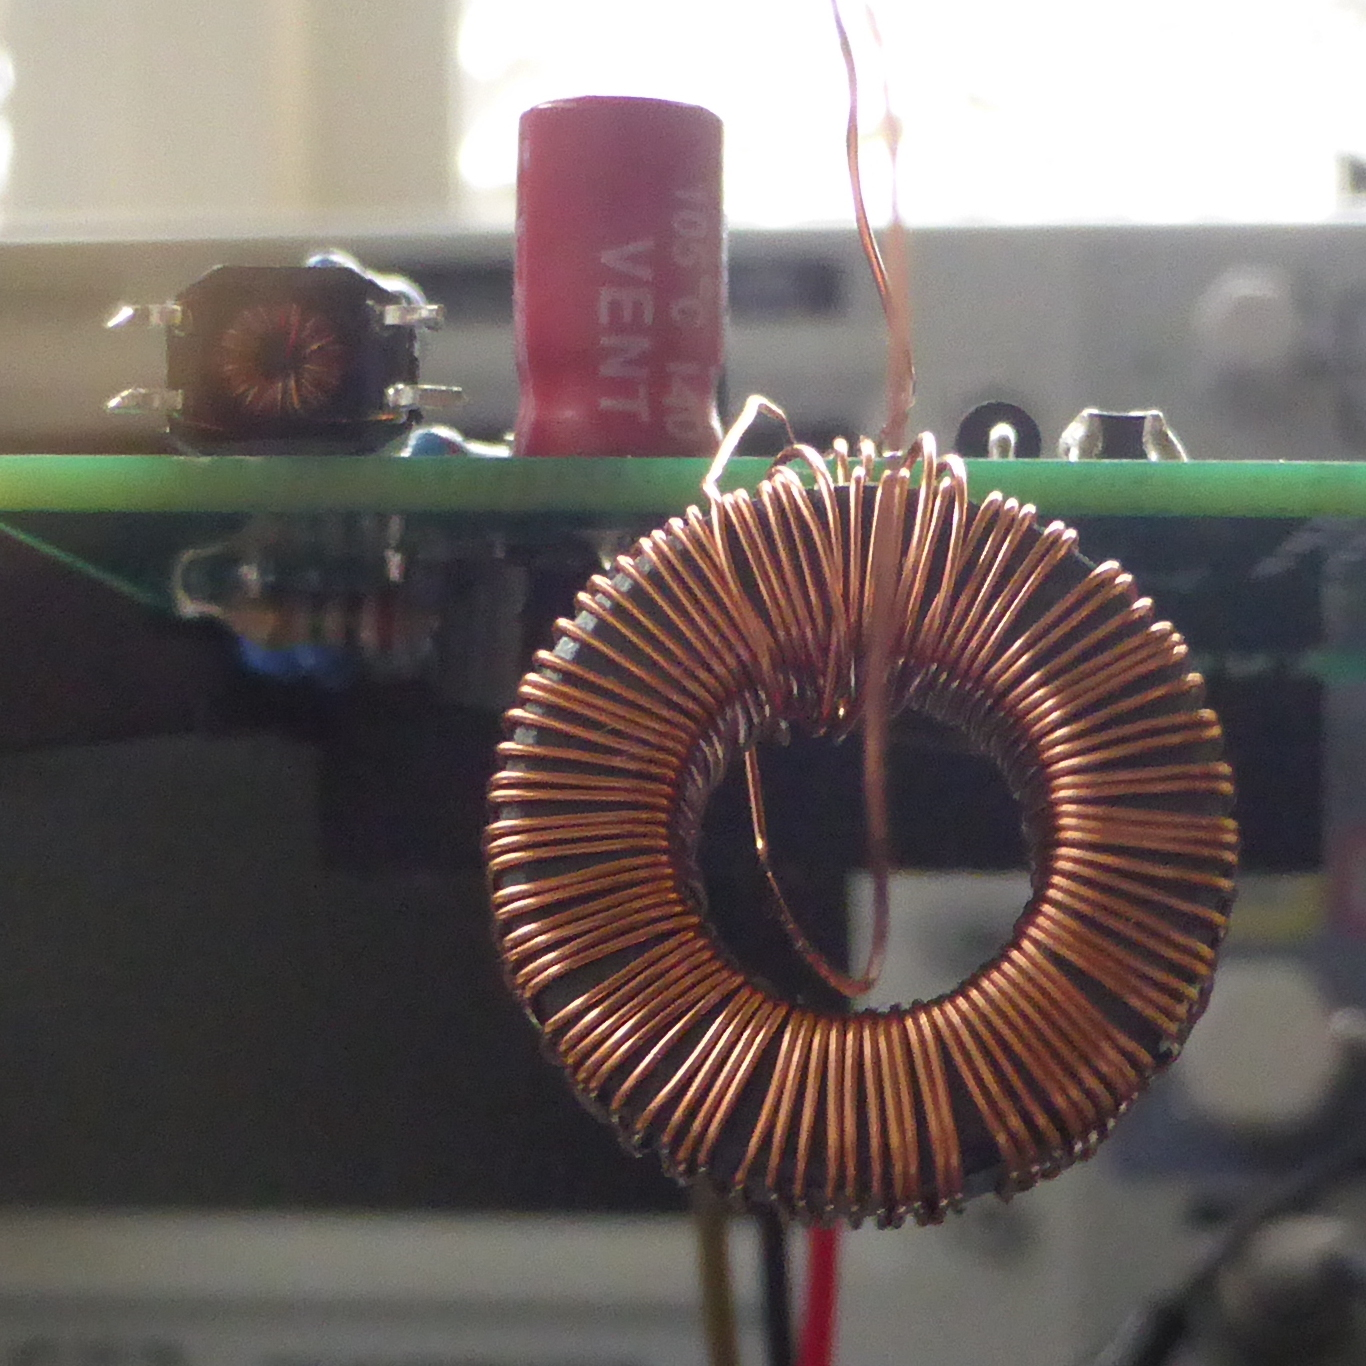
\includegraphics[height=5cm]{inductors}
  \caption[Inductors]{SMD common-mode choke (left) and hand-wound
    coupled inductors (right)}
\end{figure}


Much later into the project, when I managed to get the RP2040 to use
the osborne's clock signal to run at \qty{96}{\MHz}, the increased
power draw highlighted a flaw in my choice of a tiny common-mode choke
for the power inductor - it was too small. When the inductor reached
saturation, the converter started drawing much more current and its
output dropped substantially. It took me quite a while to figure this
out, but the tell-tale sign was the small \qty{0}{\V} ``front porch''
visible at the anode of the diode after the MOSFET turned off but
before current started to flow through the diode.

\begin{figure}
  \centering
  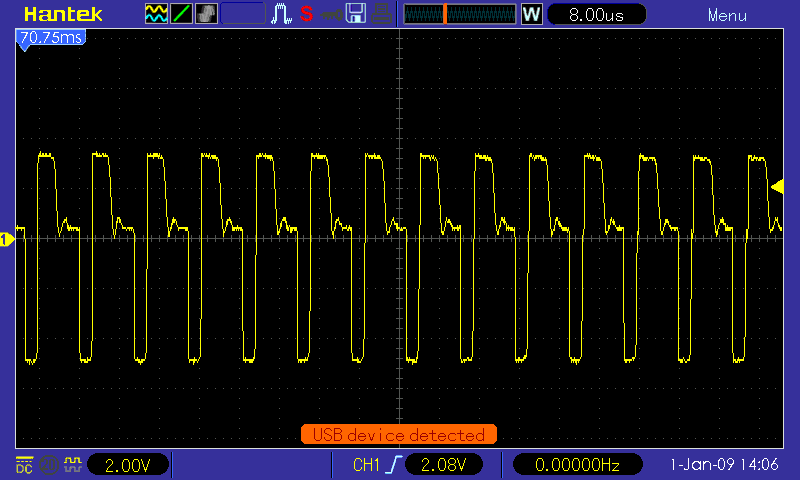
\includegraphics[height=3.5cm]{pic_23_3}\hfill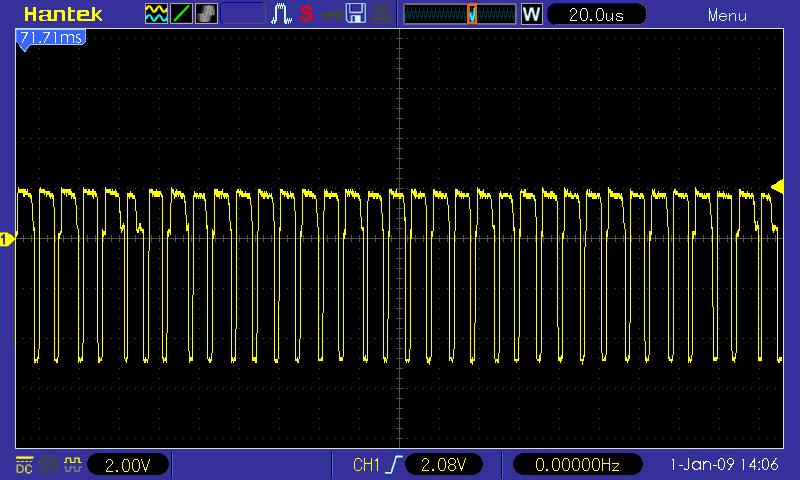
\includegraphics[height=3.5cm]{pic_23_4}
  \caption[Voltage traces with SMD choke]{Diode anode voltage
    vs. time with SMD choke - On left operating normally, on right
    with saturation issue (different horizontal scale)}
\end{figure}

\begin{figure}
  \centering
  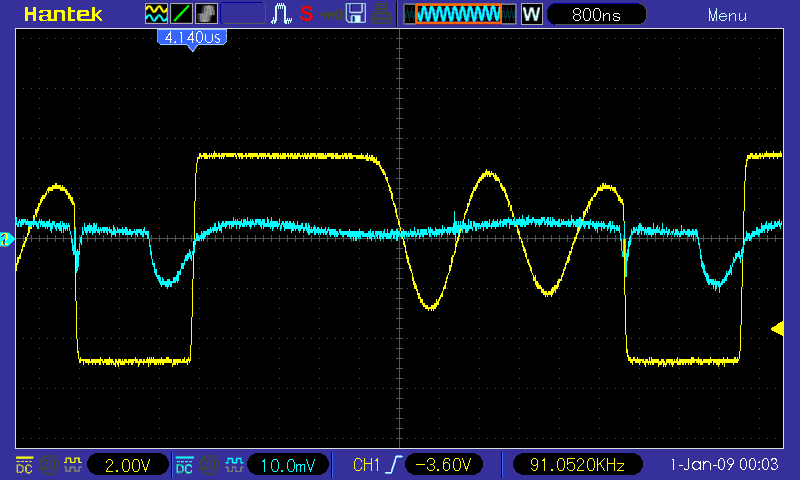
\includegraphics[height=3.5cm]{pic_25_1}\hfill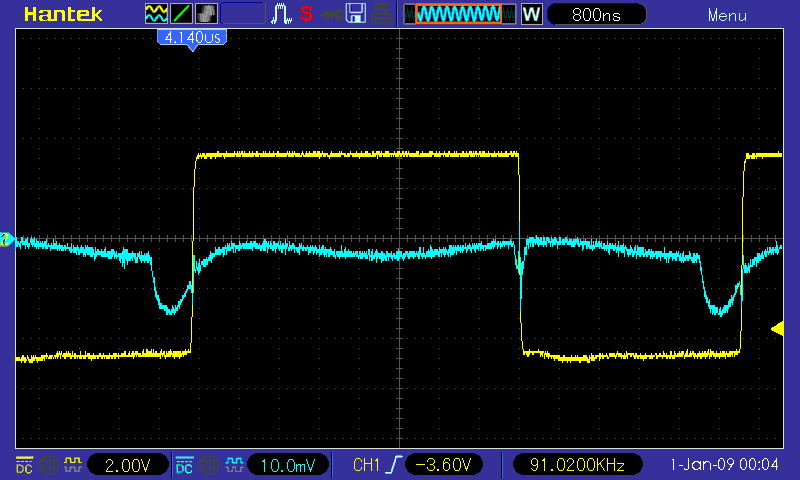
\includegraphics[height=3.5cm]{pic_25_4}
  \caption[Voltage and current traces with handwound inductors]{Diode
    anode voltage vs. time (yellow) and voltage across \qty{0.1}{\ohm}
    shunt (blue) with hand-wound inductors - On left under light load (in
    DCM) and on right under high load (in CCM)}
\end{figure}

\subsection{Processor}

The microcontroller we used was the RP2040, because I already had one
spare from another project. It is almost certainly more powerful than
we need, but having a more powerful processor allows more room for
inefficiencies when programming, and the ability to implement
additional functionality.

The RP2040 has some interesting features, the foremost of which are
that it contains 2 cores, it has 2 banks of 4 ``PIO'' (Programmable
I/O) state machines, and that it has a USB 2.0 controller and a USB
1.1 PHY. These features, along with its \qty{264}{\kibi\byte} of RAM,
make it very capable in this application.

The microcontroller contains its own ring oscillator, which is used
when debugging and programming the flash, as well as the hardware to
support a crystal oscillator, which is instead fed with the
\qty{4}{\MHz} clock given to (but not used by) the floppy drives.

\subsection{I/O}

The Osborne 1 uses TTL chips, which use \qty{5}{\V}, while the RP2040
is designed for the CMOS world, and can only handle up to
\qty{3.3}{\V}. Additionally, the Osborne 1's disk drives and
controller use ``open-collector'' chips on their outputs, which either
short their output to ground or leave it floating. This would be great
if we weren't planning to connect the physical drives as well, as we
could connect the inputs directly to the RP2040 and use its internal
pull-ups, but because we want to have the disk drives attached we need
a diode on the inputs, so the RP2040's side can be pulled down but not
up. The open-collector I/O does however make it very easy to
level-shift the outputs of the RP2040, using only a resistor (which
may not actually be required) and an NPN transistor, with the side
effect of inverting the signal.

\subsection{PCB}

I had initially planned to make the PCB for this project at home using
some copper-clad board and photosensitive paint, but it turned out
that I couldn't even create a simple PCB after 2 attempts because I
didn't realy know how to use the paint, so because of this I decided
to order the PCBs online from JLCPCB.

When I got the PCBs from JLCPCB, and the parts from Mouser, I realised
after assembling most of one PCB that I had failed to consider the
physical constraints imposed by the Osborne 1, and the board could not
fit inside it. Despite this, I was able to solder a header on the
output side of the board and plug it in backwards, allowing me to test
the power supply, and I was also able to use the debugger on the
RP2040 to test that I could program it.

Because the first design of the board was... bad, I decided to create
a second version of the PCB, this time taking into consideration the
fact that I was going to get it printed by a commercial manufacturer
who would make vias at no additional cost and has their design
tolerances listed. I also changed the parts supplier from Mouser to
LCSC, as they had the SMD pin headers that the new board needed, as
well as just generally having cheaper components. The new board also
used some SMD resistors, an SMD version of the TL494, and SMD signal
diodes and transistors, allowing a size reduction of more than two
times while most of the parts remained the same. Another one of the
changes I made between the versions was to change the RP2040's
footprint to have longer solder pads, so that it could be
hand-soldered more easily.

\begin{figure}
  \centering
  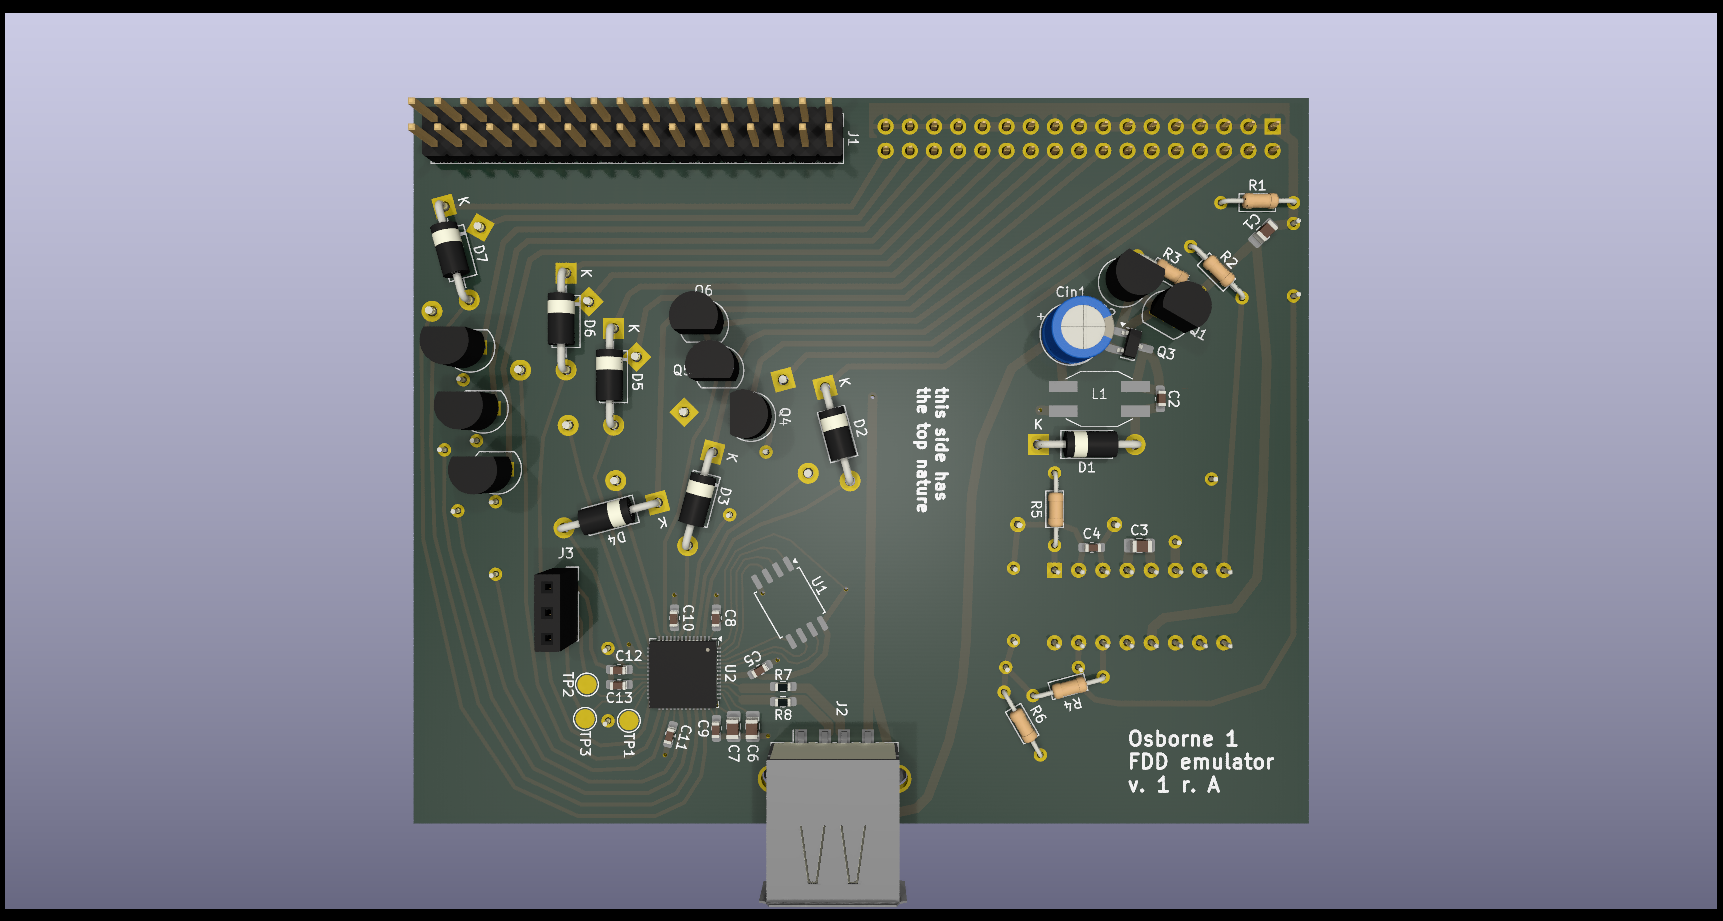
\includegraphics[height=5cm]{pcb-v1}
  \caption{Render of first version of PCB}
\end{figure}

\begin{figure}
  \centering
  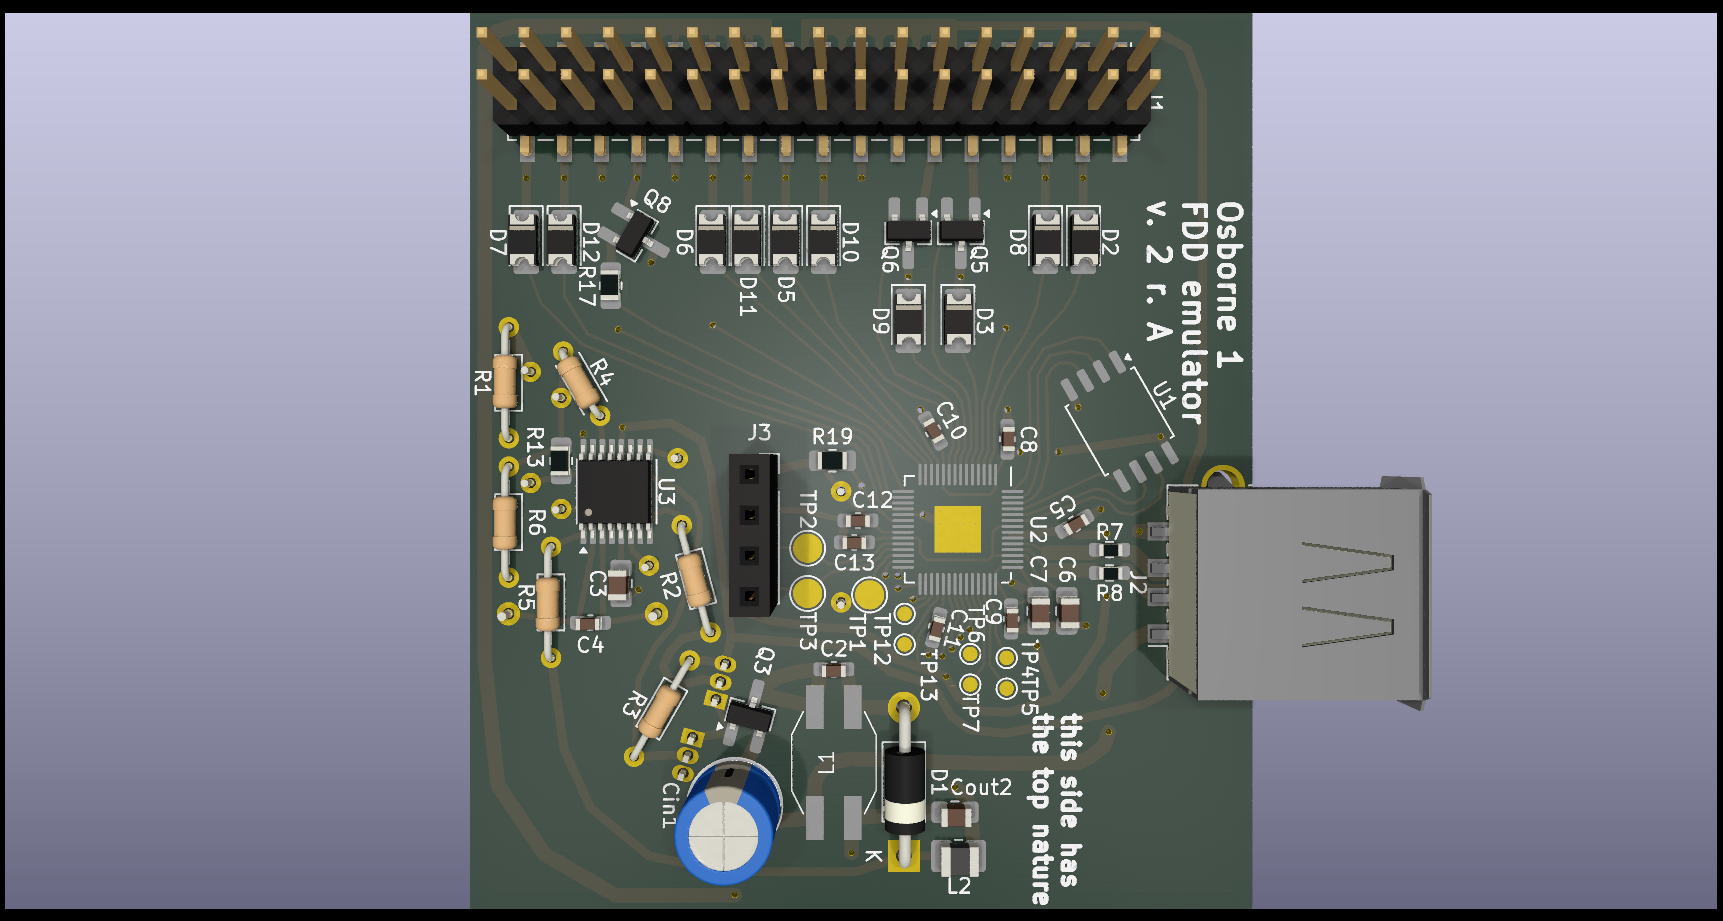
\includegraphics[height=5cm]{pcb-v2}
  \caption{Render of second version of PCB}
\end{figure}

\section{Software}

\subsection{Folly}

While I was waiting for the first version of the boards to arrive, I
decided to write a program I could run on an Arduino Uno to debug and
program the RP2040 and the flash memory respectively. This turned out
to be folly, however, as after writing about half of the program I
realised that OpenOCD would work to do all that on an SBC I already
had (it should work on any linux machine with GPIO) with minimal
configuration, although I suppose the extra practice in C programming
didn't hurt.

\subsection{GPIO}

The first program I wrote was a very simple one which simply toggled
every second (for the first version) or each (for the second version)
GPIO pin twice every three clock cycles. This was actually quite
useful for testing that the RP2040 was soldered in correctly, and that
the RP2040 could execute off of the flash memory when the board was
plugged into the Osborne 1.

When testing the emulation program for the first time, I ran into
trouble with GPIO pin directions, which was a minor stumbling block,
but I overcame it pretty easily.

\subsection{PIO}

The PIO on the RP2040 is constructed of 2 banks with 32 half-words of
instuction memory and 4 state machines each, which can write to the
GPIO pins every cycle. The main limitations of the PIOs are the
limited instuction set of 9 instructions and the limited instuction
memory. Despite this, it is still possible to create programs which
use basic logic to encode data as FM and MFM.

Initially the PIO programs were meant to run freely and be stopped and
started when required, but I later realised that the timing precision
required would not be acheivable as the main processors only knew the
time to the nearest \qty{2}{\us}. Because of this I modified the
programs heavily to use the PIO's IRQ system to switch between sending
``raw'' data (required for address marks) and modulating the data.

An interesting feature of the PIO is that it has 5 extra bits for each
instruction which it can use either to specify a delay to wait for
after execution or some pins to set before/during execution, which is
very useful for timing and reducing the number of instructions used.

\begin{figure}
\begin{verbatim}
.program readFM_irq
.side_set 1 opt
; irq-driven
; clock 2 MHz
delay:
  mov x status                 [1]; 11
normal:
  nop                          [2]; 13 
.wrap_target
  pull ifempty noblock  side 1 [1]; 0
  nop                   side 0 [5]; 2
  out pins 1                   [1]; 8
  jmp !osre delay       side 0    ; 10
  jmp !x normal                [1]; 11
  irq set 4                       ; 13
  wait 1 irq 5                    ; -1
.wrap
\end{verbatim}
  \caption{An assembly program for the PIO that will output some data,
    then cause an interrupt and wait on another when it runs out of data}
\end{figure}

The PIO has a few quirks, these include that its program counter
cannot be directly written to, meaning that the easiest way to change
it is to give it a jump instruction to execute, as well as that the
pins are all set to be inputs by default, so you need to use one of
the state machines to set the pins to outputs.

\subsection{Memory}

One of the things I spent quite a while thinking about was how to
allocate memory for storing the data on the disks without wasting too
much on metadata. After doing a bit of research I took some
inspiration from the buddy system and decided that I would have 3
different sizes of memory blocks, each being 3 times larger than the
last. The smallest size was 8 bytes, and can hold 3 bytes of data, the
second was 24 bytes, and can hold 19 bytes of data, and the largest
was 72 bytes and can hold 67 bytes of data. The 5 missing bytes in
each block contains a one-word pointer and a one-byte type, although
this could concievably be shrunk to 3 or 4 bytes using a bit field.

Each track is represented in memory by a linked list of blocks, and
each block contains either 3, 19, or 67 bytes of data; a byte and a
number of times it is repeated, or some raw data and sometimes an
extra byte. The repeated byte is useful for representing gaps and sync
bytes, and the raw data can represent address marks, which are
explained in section~\ref{subsubsec:am}.

In order to be able to allocate memory, the program needs to be able
to keep track of the free memory, which is stored in a sorted linked
list. Newly freed memory is placed in a seperate list, which is later
sorted and merged into the main list. Each of the different sizes of
blocks has its own linked lists, but the program will automatically
decide to split up the largest size of blocks when there is a deficit
of the smaller blocks, and merge these blocks together when there is
an excess.

\subsection{USB}

For a short period of time, I thought that I might try to create my
own USB driver because it seemed like a hassle to learn someone else's
library, but I decided against this after reading more about USB and
how complicated it is, as well as just thinking about how complicated
filesystems are. Because of this, we were going to use TinyUSB stack,
however we have not started implementing USB at time of writing. We
are planning on running USB on processor 1 while the floppy drive
emulator runs on processor 0, to allow us to read data from the USB
stick and manipulate it to some degree while emulating a floppy drive,
which is important as an MFM disk may not completely fit in memory, so
its tracks must be streamed from the USB mass storage device. Whether
or not the regular interrupts and other tasks on processor 0 would
slow down USB transfers is unknown, but by processing the data on both
cores we can hopefully acheive a speed-up, as each sector is loaded
and the CRC calculated using one processor while the other one places
the last sector into a linked list.

\subsection{Images}

Most of the disk images floating around on the internet are stored in
the ImageDisk format, which was created by Dave Dunfield for his
ImageDisk disk imaging program he dubbed ``created by
necessity''. Because of this it is a somewhat strange, but simple,
format which should not be very difficult to parse, however we have
not programmed this yet as we haven't written the code to read off of
USB mass storage yet.

A slight problem with the ImageDisk format is that it was designed for
archiving data, rather than exact reproduction of the disk, so it
doesn't contain much formatting information such as gap sizes, or have
any way to represent bytes with missing clock bits, as these are not
usually significant in operating systems, and missing clock bits will
go unnoticed by the computer unless they cause the FDC to report an
error. This presents a problem if we want to faithfully reproduce a
floppy drive down to the errors, as we will need a way to store
abnormal bytes and incorrect CRCs. As of yet we have no plan on how to
go about this, but we could potentially create our own format based on
the way that we store data in memory.

\section{Format}

Note that this section relates to IBM 3740 and IBM System 34 and
similar formats (including the Osborne formats).

\subsubsection{MSB-first}

Something important about the format of floppy disks that it doesn't
seem is mentioned very often is that the bytes are transmitted
MSB-first (I assumed that they were transmitted LSB-first but when
looking at datasheets LSB-first didn't make sense with the bits they
said were missing in the MFM address marks).

\subsection{FM}

Data is stored on floppy disks as a series of transitions, as the head
cannot pick up any ``DC'' (constant) component of the magnetic field
on the disk. Additionally, as the disk may spin at different speeds in
different drives, there must be some way to differentiate between a
missing transition and the time between two transitions. We need to
recover a ``clock'' signal. The way that the Osborne 1 does this is by
feeding the signal from the drive, which generates a pulse for every
transition, into a circuit which outputs a clock signal synchronised
with the last pulse it recieved. The problem with this is that if the
data we write to the disk contains a special pattern, such as a lot of
zeros, the disk will contain no transitions and our clock could drift
out of sync, inserting or deleting data. So, what we do is we just add
an extra transition between every bit of data that we send. This is
dubbed ``FM'', as this method produces one frequency when the data bit
is 0 (no transition) and double the frequency when the data bit is 1
(transition); in the case of the Osborne 1 the frequency of 0 is
\qty{125}{\kHz} and the frequency of 1 is \qty{250}{\kHz}. Outside of
data storage this is also known as Differential Manchester Encoding,
or as a run-length limited encoding \(RLL \left(0,1\right)\). The
problem with FM is that there is a limit on the highest frequency we
can record on a floppy disk, and FM isn't particularly economical in
this aspect.

How can we do better? By reducing the number of transitions! If we
just get rid of all the ``clock pulses'' that are next to ``data
pulses'' we can halve the fundemental frequency for a given data rate,
or equivalently double the data rate for a given fundemental
frequency. Because this is slightly different to FM, it is called
``MFM'', for ``Modified Frequency Modulation'' (it is also \(RLL
\left(1,3\right)\)). The drawback of this is that encoding and
decoding it is more complicated, but it's well worth the cost to get
double the data storage on the same disks. The sequence 11 still has a
frequency of \qty{250}{\kHz}, but so does the sequence 00. The
sequence 1010 has a frequency of \qty{125}{\kHz} and the sequence 100
has a frequency of just over \qty{166}{\kHz}.

\subsubsection{AM}
\label{subsubsec:am}

One of the more interesting things about the IBM 3740 and IBM System
34 formats is that the IBM 3740 format uses address marks (which mark
the beginnings of data and metadata sections) with missing clock bits,
and the IBM System 34 format preceeds the address marks with 3 bytes
missing a clock bit. This gives the FDC the ability to find them
amongst whatever strange data might be on the disk, but also
complicates the job of a floppy drive emulator. In order to be able to
send address marks our program uses two of the PIO state machines
running different programs, which synchronise with each other to allow
the emulator to send an address mark followed by regular bytes,
without the processor having to add the clock signal to regular bytes.

\subsection{Metadata}

Each sector on the floppy disk has a small amount of metadata
associated with it, almost all of which is stored in what is known as
the ``ID field''---the only part which isn't is whether the data is
deleted or not, which is stored in the data (or deleted data) address
mark. The ID field stores the track number, the side number (only 0 or
1), the sector number, and the sector length (as a power of 2 times
128). The ID and data fields both also contain a 16-bit CRC of all of
the data from the start of the last address mark, which uses the
polynomial \(x^0 + x^5 + x^{12} + x^{16}\), and is also known as
CRC-16-CCITT.

There is also a short preamble that starts when the index pulse
begins, which is sent by the floppy drive when a small hole punched in
the floppy disk is detected at a certain position by a photogate-like
device. All that this preamble contains is an index address mark,
which presumably serves to verify that the drive's head is not somehow
reading part of the disk which shouldn't even be exposed as the index
hole goes past.

\subsection{Gap}

Formatted disks include gaps, where no data is stored, that are placed
between data fields and ID fields, as well as between the end and
start of the disk. The gaps are numbered 0 through 4, with gaps 2 and
3 appearing once for each sector. The FD179X chips and their clones
have minimum size requirements for most of the gaps, except for gap 0
which occurs after the index pulse (at the start of the disk) and is
nominally 40 bytes in FM and 80 in MFM, and gap 2, which must always
be 11 bytes in FM and 22 in MFM. Interestingly, in FM the gaps contain
the byte 0xFF (0b11111111), while in MFM they contain 0x4E
(0b01001110). This is perhaps because in MFM the byte 0xFF could be
confused with the byte used for the sync after gaps 2 and 3, which is
0x00. In MFM this sync section is followed by 3 bytes of 0xA1 missing
the clock transition between bits 4 and 5 in the sectors, or 0xC2
missing the clock transition between bits 3 and 4 in the preamble. The
flexibility in gap lengths allowed by these chips made it possible for
designers to make formats that squeezed more actual data into the disk
by missing out parts of the gaps - this could save 19 bytes per sector
compared to the IBM 3740 format and 34 bytes per sector compared to
the IBM System 34 format, plus a few hundred more by shortening gap 4,
which would reduce the tolerance for fast disks but allow a few more
kilobytes to be stored.

\end{document}
